%
% Chapter 4
%
\chapter{Solution Architecture}\label{chap:architecture}

The present chapter covers the system's components, their interactions, and the underlying technologies used to implement the solution. The architecture is designed to ensure data integrity, security, and scalability while providing a seamless user experience. We will cover the concept of a multiplatform application, how it functions, the various solutions available, and a detailed discussion of the chosen technology stack, specifically React Native with the Expo\cite{Expo} platform.

\section{Architecture Overview}\label{sec:architecture-overview}

The architecture of the \texttt{DiGo Certify} system is designed to be modular, scalable, and secure. The system~\ref{fig:architecture-overview} is divided into two main layers: the mobile application layer and the fully distributed layer. Each layer has specific responsibilities and interacts with the others to deliver the desired functionality.

\subsubsection{Mobile Application Layer}

The mobile application layer consists of the DiGo Certify application, which is built using React Native and Expo. This application is responsible for the user interface and handles interactions with the end-users. The choice of React Native ensures that the application is cross-platform, providing a seamless experience on both iOS and Android devices. The application allows users to register, authenticate, and manage their certificates. It communicates with the distributed layer to store and validate these certificates on the Ethereum blockchain.

\subsubsection{Fully Distributed Layer}

The fully distributed layer is implemented using the Ethereum blockchain. It consists of smart contracts written in Solidity, which handle the storage and validation of academic certificates. This layer leverages the security and immutability of the blockchain to ensure the integrity of the certificates. The interaction between the mobile application and the blockchain is facilitated by a provider, such as Hardhat, which helps in deploying and managing the smart contracts.

\paragraph{}
Below is a high-level diagram of the DiGo Certify architecture:

\begin{figure}[H]
    \centering
    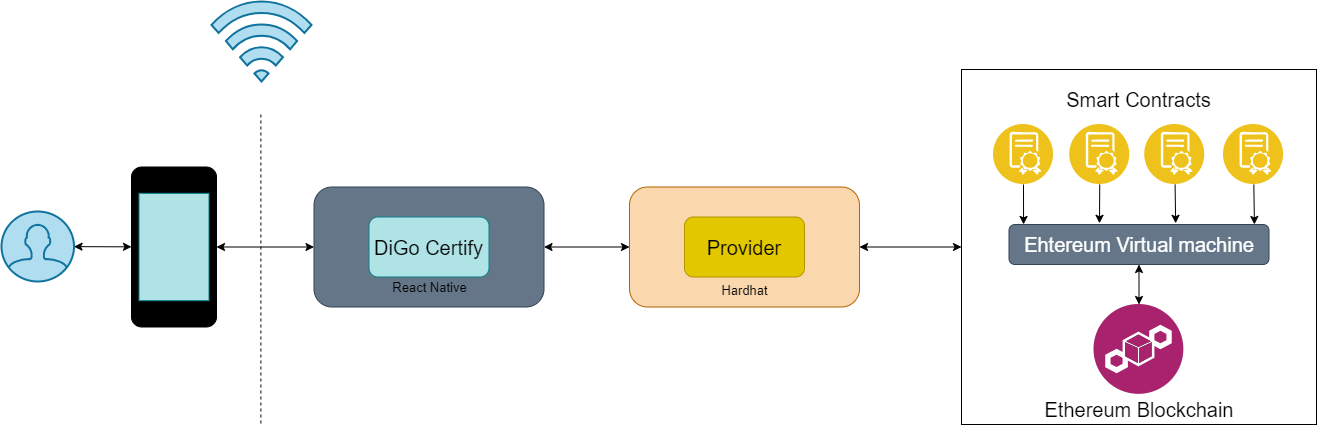
\includegraphics[width=1\textwidth]{../diagrams/architecture-overview.drawio.png}
    \caption{Architecture Overview Diagram (inspired by~\cite{geeksforgeeks-dApps}).}
    \label{fig:architecture-overview}
\end{figure}

\section{Fully Distributed Environment}\label{sec:fully-distributed-environment}

The fully distributed environment of the DiGo Certify system leverages blockchain technology to create a secure, decentralized, and transparent platform for managing academic certificates. By using the Ethereum blockchain, the system ensures that certificates are immutable and verifiable by any third party, thereby eliminating the risk of fraud and enhancing trust in the certification process.

\subsection{Smart Contracts on Ethereum}

At the core of the distributed environment~\ref{fig:architecture-overview} are the smart contracts deployed on the Ethereum blockchain. Smart contracts are self-executing contracts with the terms of the agreement directly written into code. In the context of DiGo Certify, these smart contracts handle the issuance, validation, and storage of academic certificates. Each certificate is represented as a unique digital asset on the blockchain, and its authenticity can be easily verified by checking the blockchain records.

The smart contracts are written in Solidity, a statically-typed programming language designed for developing smart contracts that run on the Ethereum Virtual Machine (EVM). The key functions of these smart contracts include:

\begin{itemize}
    \item \textbf{Certificate Issuance:} This function allows authorized entities, such as educational institutions, to issue certificates to students. The institution submits a transaction to the smart contract, including details such as the student’s name, course, and date of completion. Upon verification, the smart contract records the certificate on the blockchain.

    \item \textbf{Certificate Validation:} This function enables third parties, such as employers, to verify the authenticity of a certificate. By querying the blockchain, they can confirm that the certificate was indeed issued by a legitimate institution and has not been altered.

    \item \textbf{Certificate Storage:} Certificates are stored in a decentralized manner on the blockchain. This ensures that they are \textit{tamper-proof} (i.e., they cannot be altered or manipulated) and can be accessed by anyone with the appropriate permissions.

\end{itemize}

\subsection{Ethereum Virtual Machine (EVM)}

The Ethereum Virtual Machine (EVM) is a decentralized computing environment that executes smart contracts on the Ethereum network. The EVM ensures that the execution of smart contracts is consistent and secure across all nodes in the network\cite{EVM}. This decentralized nature of the EVM makes it highly resistant to hacking and fraud, as any attempt to alter a certificate would require the attacker to gain control of a majority of the network’s computing power, which is practically impossible. Once a certificate is recorded on the blockchain, it cannot be altered or deleted, ensuring that the certificates remain trustworthy and verifiable indefinitely. Additionally, all transactions on the Ethereum blockchain are publicly accessible, providing a transparent record of certificate issuance and validation, which enhances trust in the certification process.

\subsection{Provider (Hardhat)}

Hardhat is a comprehensive development environment for Ethereum software, providing an array of tools for compiling contracts, running tests, and deploying them to the blockchain. It significantly simplifies the development and deployment process, making it easier to manage the smart contracts that underpin the DiGo Certify system.

During the development phase, Hardhat is used to compile Solidity code into bytecode that can be executed by the Ethereum Virtual Machine (EVM). It allows developers to write and run tests, ensuring that smart contracts behave as expected. Hardhat also provides scripts for deploying smart contracts to the Ethereum network, making the deployment process straightforward and repeatable.

In addition to its development capabilities, Hardhat also plays a role in facilitating the interaction between the mobile application and the blockchain during the execution phase. This ensures smooth and secure communication between the components of the DiGo Certify system. Although primarily a development tool, Hardhat's robust features and integration capabilities make it useful throughout the lifecycle of the smart contracts.

In the context of the DiGo Certify system, Hardhat serves as a development and deployment environment, while also supporting interaction with the blockchain during execution. It's important to note that other tools and services, such as Infura or Alchemy, can be used as blockchain providers during execution. These services offer additional capabilities, such as scalable node infrastructure and advanced monitoring, but in our implementation, Hardhat has proven sufficient for both development and interaction purposes.

\subsection{Security}

Security and scalability are critical considerations in the design of the DiGo Certify system. The Ethereum blockchain’s inherent security features, such as its decentralized consensus mechanism and cryptographic algorithms, providing a robust foundation for secure certificate management. Additionally, the use of smart contracts ensures that certificate issuance and validation processes are automated and tamper-proof\cite{Wood2014}.

\section{Mobile Application}\label{sec:mobile-application}

\subsection{Multiplatform Application}\label{sec:multiplatform-application}

A multiplatform application is designed to run seamlessly on multiple operating systems, such as iOS and Android, using a single codebase. This approach significantly reduces development time and costs while ensuring a consistent user experience across different devices. The core idea is to write the code once and deploy it across multiple platforms, which is particularly beneficial for applications that need to reach a broad audience.

\subsubsection{Functionality and Operation}

Multiplatform applications leverage frameworks that provide tools and libraries to facilitate cross-platform development. These frameworks abstract away the differences between the various platforms, allowing developers to focus on building features rather than dealing with platform-specific nuances. The primary goal is to achieve native-like performance and look-and-feel while maintaining a shared codebase.

\subsubsection{Available Solutions}

Several frameworks are available for developing multiplatform applications, each with its own set of features and trade-offs. The most notable ones include:

\begin{itemize}
    \item React Native\cite{ReactNativeBook}
    \item Flutter\cite{Flutter}
    \item Kotlin Multiplatform Mobile (KMP)\cite{KMP}
\end{itemize}

\subsubsection{React Native}

React Native is a popular open-source framework developed by Facebook. It allows developers to build mobile applications using JavaScript and React, a widely-used library for building user interfaces. React Native bridges the gap between web and mobile development by enabling code reuse across platforms while providing near-native performance\cite{ReactNativeBook}.

\paragraph{Key Features:}

\begin{itemize}
    \item \textbf{Component-Based Architecture:} Enables modular and maintainable code.
    \item \textbf{Hot Reloading:} Allows developers to see changes in real-time without recompiling the entire application.
    \item \textbf{Rich Ecosystem:} A vast collection of libraries and tools that streamline development.
    \item \textbf{Community Support:} Extensive community contributions and support.
\end{itemize}

\subsubsection{Flutter}

Flutter, developed by Google, is another powerful framework for building natively compiled applications for mobile, web, and desktop from a single codebase. It uses the Dart programming language and provides a rich set of pre-designed widgets to create highly customizable interfaces\cite{Flutter}.

\paragraph{Key Features:}

\begin{itemize}
    \item \textbf{Hot Reload:} Similar to React Native's hot reloading, enabling quick iterations.
    \item \textbf{Expressive UIs:} Rich set of customizable widgets.
    \item \textbf{Performance:} Compiled directly to native code, which can lead to better performance.
\end{itemize}

\subsubsection{Kotlin Multiplatform Mobile (KMP)}

KMP, developed by JetBrains, allows developers to use Kotlin for developing iOS and Android applications. It focuses on sharing code, particularly business logic, while allowing platform-specific code where necessary\cite{KMP}.

\paragraph{Key Features:}

\begin{itemize}
    \item \textbf{Code Sharing:} Share common code across platforms while writing platform-specific code when needed.
    \item \textbf{Native Performance:} Utilizes native components and performance optimizations.
\end{itemize}

\subsection{Chosen Solution: React Native with Expo}

For the \texttt{DiGO Certify} application, we chose React Native with the \texttt{Expo} platform. This decision was influenced by several factors, including our team's familiarity with JavaScript and React, the maturity and stability of the React Native ecosystem, and the added benefits provided by Expo\cite{Expo}.

To make an informed decision, we compared several frameworks, including Flutter and Kotlin, based on various parameters~\ref{tab:comparison}.

\begin{table}[h]
    \centering
    \label{tab:comparison}
    \caption{Comparison of Flutter, React Native, and Kotlin.\cite{RNvsFluttervsKMP}}
    \begin{tabular}{|p{2.5cm}|p{4cm}|p{4cm}|p{4cm}|}
        \hline
        \textbf{Parameter}         & \textbf{Flutter}                           & \textbf{React Native}                             & \textbf{Kotlin}                                                        \\ \hline
        \textbf{Ease of Coding}    & Widget-based, reactive framework (Dart)    & JSX and JavaScript, component-based (React)       & Concise, expressive, reduces boilerplate (Kotlin)                      \\ \hline
        \textbf{Scalability}       & Good scalability, reactive architecture    & Scales well, may need native modules              & Excellent scalability, especially for large codebases                  \\ \hline
        \textbf{Performance}       & High performance, compiled language (Dart) & Near-native performance, native modules if needed & Efficient performance, native language for Android                     \\ \hline
        \textbf{Learning Curve}    & Moderate, widget-based approach            & Relatively easy for JavaScript developers         & Moderate, especially for those familiar with Java                      \\ \hline
        \textbf{Popularity}        & Growing rapidly, gaining popularity        & Widely adopted, mature, and well-established      & Highly popular for Android development                                 \\ \hline
        \textbf{Stability}         & Stable, regular updates and improvements   & Stable, backed by Facebook and active community   & Stable, regular updates and improvements                               \\ \hline
        \textbf{Types of App Dev}  & Cross-platform focus for consistent UI     & Cross-platform, leverages JavaScript expertise    & Primarily for native Android; Kotlin Multi Platform for cross-platform \\ \hline
        \textbf{Community Support} & Growing community support                  & Large and active community support                & Strong support, especially in the Android community                    \\ \hline
    \end{tabular}
\end{table}


React Native’s component-based architecture aligns well with our need for a modular and maintainable codebase. Our team’s existing knowledge of JavaScript and React significantly reduced the learning curve, allowing us to quickly become productive and focus on delivering features. Compared to Flutter and Kotlin, React Native's learning curve is relatively easy for JavaScript developers, while Flutter requires learning Dart, and Kotlin, despite being expressive and reducing boilerplate, may be more moderate for developers familiar with Java.

In terms of performance, React Native provides near-native performance, ensuring that our application runs smoothly on both iOS and Android\cite{react-native-performance}. This is similar to Flutter~\ref{tab:comparison}, which offers high performance through its compiled language, Dart, and Kotlin, which provides efficient performance for native Android development. However, React Native can scale well with the potential need for native modules, providing flexibility in development.

The framework’s rich ecosystem of libraries and tools further accelerated our development process, providing pre-built components and solutions that we could easily integrate into our application. The extensive community support for React Native ensured that we had access to numerous resources, tutorials, and third-party libraries, which proved invaluable during the development process. This support network allowed us to quickly troubleshoot issues and implement best practices, contributing to a more efficient development cycle. While Flutter's community is rapidly growing, React Native's community is already large, mature, and well-established, and Kotlin also enjoys strong support, especially in the Android community.

Expo enhances React Native by offering a suite of tools and services that simplify development\cite{Expo}. With Expo, we benefit from an integrated environment for developing, building, and deploying React Native applications. The platform’s managed workflow handles many of the complexities of building and deploying mobile applications, allowing us to focus on developing features rather than dealing with infrastructure. Expo’s easy setup and configuration process streamlined our project initialization, while its over-the-air update capability enables us to push updates to users without requiring a full app store review process.

The development workflow for DiGo Certify using React Native and Expo involves several key steps. Initially, we set up the project with Expo CLI, which provides a streamlined setup process and essential tools. We then focused on building the application UI using React Native’s component-based approach. This method allows us to create reusable UI elements that help maintain consistency and simplify development.

For integrating blockchain functionality, we implemented smart contracts in Solidity and connected them with the React Native application through ethers.js. This integration enables secure interactions with the Ethereum blockchain, allowing for the storage and validation of academic certificates.

Testing and debugging are facilitated by Expo’s built-in tools, which allow us to test the application on various devices and simulators. This ensures that our application performs well across different platforms and devices. Finally, Expo simplifies the deployment process with its build and publish services, allowing us to distribute the application through app stores seamlessly.

In summary, the choice of React Native with Expo for DiGo Certify provides a robust, efficient, and scalable solution for developing a secure and user-friendly multiplatform application. This architecture leverages modern technologies to meet the needs of our diverse user base, ensuring a high-quality user experience across all supported devices.

\section{Proposed Model}

\subsection{Certificate Issuance}

Initially, a student or alumni requests a certificate from the OnchainID~\cite{ONCHAINID} system. The system checks whether the requester has an existing OnchainID. If it exists, the system proceeds to verify the associated claims and sends the certificate to the DiGo Certify application. The application then submits the certificate to the blockchain for validation and secure storage. Once the certificate is successfully submitted, it is delivered back to the student or alumni. In cases where the OnchainID does not exist, the system initiates the creation of a new identifier. This involves sending a certificate emission request to the Admin for approval. Upon receiving the request, the Admin emits the certificate and submits it to the blockchain. After the submission, the certificate is sent back to the OnchainID system, which verifies the claims and delivers the certificate to the student or alumni. This process ensures that all issued certificates are securely stored on the blockchain, providing a tamper-proof and verifiable record of the certification.

\begin{figure}[H]
    \centering
    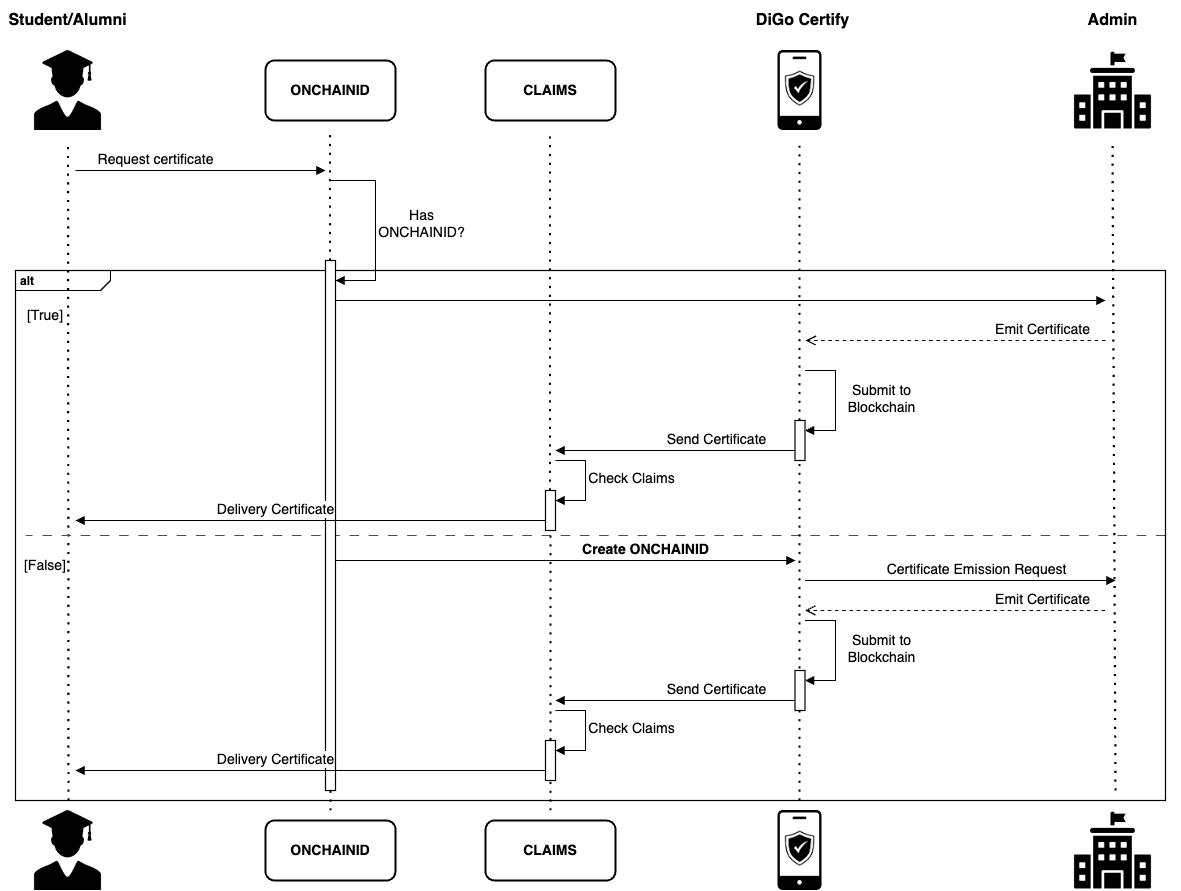
\includegraphics[width=0.6\textwidth]{../diagrams/certificate-request-diagram-sequence.png}
    \caption{Certificate Issuance.}
    \label{fig:certificate-issuance}
\end{figure}

\subsection{Requesting and Approving changes on a certificate}

The process begins with the student or alumni initiating a request for changes to their certificate. The DiGo Certify application then submits the modified certificate to the blockchain for validation. Upon processing the transaction, the blockchain provides a confirmation of the changes. This confirmation is sent back to the student or alumni, notifying them of the acceptance or denial of the requested changes. Concurrently, the Admin is notified of the requested changes. If the changes are approved, the Admin emits a new certificate with the modifications and submits it to the blockchain. The modified certificate is processed by the blockchain, completing the transaction. This process allows for the secure and transparent modification of certificates, ensuring that any changes are recorded on the blockchain and are verifiable by all parties involved.

\begin{figure}[H]
    \centering
    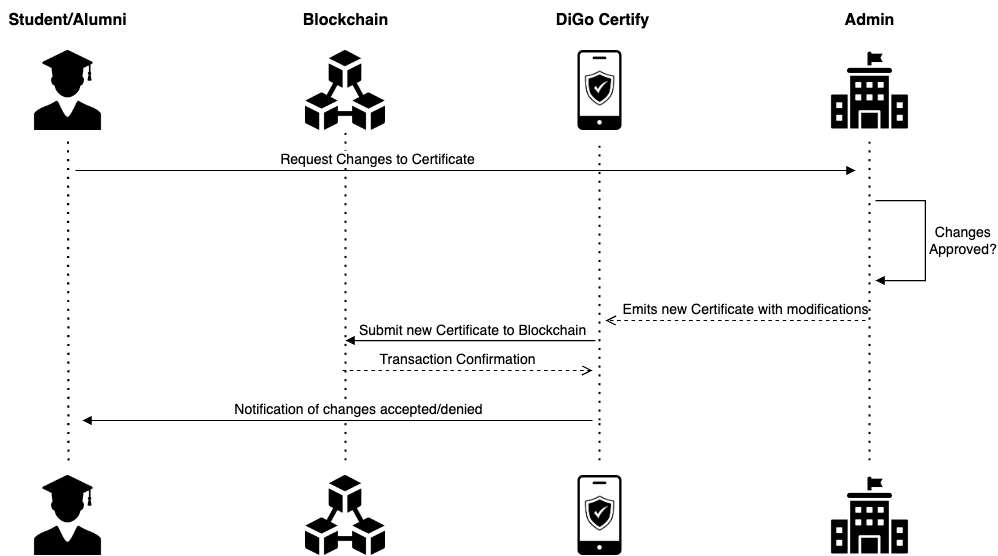
\includegraphics[width=0.6\textwidth]{../diagrams/certificate-update-diagram-sequence.png}
    \caption{Certificate update request.}
    \label{fig:certificate-update}
\end{figure}

\subsection{Certificate Validation}

When a student or alumni first provides their certificate to a third party who needs to verify its authenticity. The third party then initiates an authentication request to the DiGo application. Upon receiving the request, the DiGo verifies the certificate's authenticity by checking its records against the blockchain. This verification process ensures that the certificate has not been tampered with and is indeed issued by a recognized authority. Once the verification is complete, the DiGo Certify application confirms the authenticity of the certificate back to the third party. Subsequently, the third party can confidently rely on the certificate's validity, and the student or alumni is informed of the successful verification. This process underscores the importance of blockchain in maintaining the integrity and trustworthiness of academic certificates, ensuring that any third party can independently confirm their authenticity without relying solely on the issuing institution.

\begin{figure}[H]
    \centering
    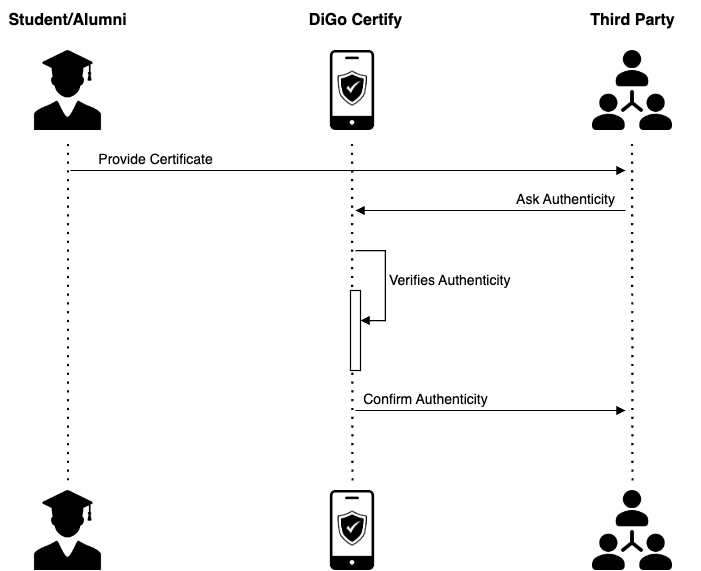
\includegraphics[width=0.6\textwidth]{../diagrams/certificate-validation-diagram-sequence.drawio.png}
    \caption{Certificate update request.}
    \label{fig:certificate-validation}
\end{figure}